\chapter{Storage Layer}\label{storage-ch}

Pinky stores both raw EEG voltage readings and calculated spectrograms. The raw
EEG data is simply a matrix with a column for each sensor (see
Figure~\ref{fig:electrodes}) and a data sample read by the sensor at each row.
Similarly, we store the spectrogram, a range of frequencies across time, as a
multidimensional array. Since matrices of floating point values represent both
raw EEG data and the spectrogram visualization, the system requires an
efficient way to store and query such large multidimensional arrays. The
storage layer meets this requirement by providing an abstraction called the
\c{StorageBackend} for storing array based data. The abstraction gives read and
write access to 2-dimensional matrices of \c{float} values. Since the
interactivity the system demands requires efficient querying of the data, we
evaluate different array based storage systems and compare the tradeoffs of
each against a simple storage system that we implement.

\section{Design}

The \c{StorageBackend} abstraction provides a thin layer over existing array
based storage systems to provide a consistent API for evaluation across
different systems. The goal is to efficiently expose read and write access to
large array based datasets. A patient EEG scan typically lasts 24 hours, but
can run for up 7 days \cite{ceeg-3}. The raw output of voltage readings yield a
file from tens to hundreds of gigabytes in size. We assume that the entire
dataset cannot always fit into the memory of the server, given that it must
concurrently respond to multiple client queries. Thus, the \c{StorageBackend}
should rely on maintaining an efficient on disk representation of the data. \\

A \c{StorageBackend} implementation must primarily handle three different
workloads. The first is data ingestion. This is a write heavy workload --
reading patient data files from disk and storing them in the system. Secondly,
spectrogram data is typically written once in a precomputation step, and saved
for later analysis. This workload is primarily read heavy, since the computed
spectrogram is much smaller in size than the raw input file.  After being
stored, efficient reads are required for an analyst to access the
visualizations.

\subsection{Ingestion Workload}

Once a patient scan is complete, the system ingests the raw data file for
analysis. The raw data is initially stored in the European Data Format (EDF)
\cite{edf}, a simple binary format for storing multichannel biological and
physical signals. During ingestion, we read the data in chunks of configurable
size from an input EDF file and convert them for storage within the system.
This workload requires the storage system to efficiently handle the addition of
large datasets. We evaluate the performance when ingesting data in
Section~\ref{storage-ch:ingestion-exp}.

\subsection{Precomputation Workload}

After ingesting a file into the system, the spectrogram for a patient is
computed, reading the raw values from the storage system. This precomputation
step is important for minimizing the latency when serving the visualization.
The precomputation calculation involves reading columns of the raw data to
perform the spectrogram calculation and writing the spectrogram matrix back to
the datastore. We describe the details of the calculation in
Section~\ref{compute-ch:design-spectrogram}. This workload requires efficient
reading of individual columns in the raw data and, similarly to the ingestion
workload, the ability to write dense matrices efficiently.

\subsection{Visualization Serving Workload}

In practice, the primary workload the storage system must handle is serving
chunks of a calculated visualization. Analysts will request data for a given
patient and time interval and need to be able to quickly have the results
rendered. This workload requires efficient reading of chunks of the matrix.

\section{Implementation}

The storage layer is implemented in C++, providing a common interface to access
array based datasets. We create a \c{StorageBackend} by inheriting from the
\c{AbstractStorageBackend} interface and implementing the methods described in
Section~\ref{storage-ch:api} using an array storage system. This design allows
us to interchange storage systems for evaluation without affecting other layers
within the overall system. To compare the tradeoffs between different array
store systems for each workload, we implement 3 versions of \c{StorageBackend}
using two existing systems, HDF5 \cite{hdf5} and TileDB \cite{tiledb} and our
own implementation as a baseline. \\

We begin by describing the API in Section~\ref{storage-ch:api} followed by a
description of each implementation in
~\cref{storage-ch:implementation-binary,storage-ch:implementation-hdf5,storage-ch:implementation-tiledb}.
The command line programs that are available for this layer are described in
Section~\ref{storage-ch:implementation-cmd}, and finally we discuss some
overall optimizations in Section~\ref{storage-ch:opt}.

\subsection{StorageBackend API}\label{storage-ch:api}

The \c{StorageBackend} API allows creating, reading, and writing arrays. Each
array corresponds to a patient's unique medical record number, their \c{mrn}.
The API is as follows:

\begin{lstlisting}
    ArrayMetadata get_array_metadata(string mrn);
    void create_array(string mrn, ArrayMetadata* metadata);
    void open_array(string mrn);
    void read_array(string mrn, int ch, int start_offset,
                    int end_offset, float* buf);
    void write_array(string mrn, int ch, int start_offset,
                    int end_offset, float* buf);
    void close_array(string mrn);
\end{lstlisting}

\subsubsection{\c{ArrayMetadata get\_array\_metadata(string mrn)}}

Each array has an associated \c{ArrayMetadata} object which describes the size
of the matrix. Specifically, \c{ArrayMetadata} stores three \c{int} values which
are necessary for the spectrogram calculation and for the client to prepare the
visualization. The values are as follows:

\begin{lstlisting}
    int fs;
    int nrows;
    int ncols;
\end{lstlisting}

\c{fs} is the frequency rate at which the sampling occurred during the EEG
scan. \c{nrows} and \c{ncols} represent the number of rows and columns in the
matrix respectively. Each array based system has a different way of storing
metadata values, thus the \c{ArrayMetadata} object provides a common interface
to access and deserialize them.

\subsubsection{\c{void create\_array(string mrn, ArrayMetadata* metadata);}}

The \c{create\_array} function takes as input a patient's medical record
number, \c{mrn} and a pointer to a \c{ArrayMetadata} object. The function is
responsible for defining the array and persisting the \c{ArrayMetadata} to
disk.

\subsubsection{\c{void open\_array(string mrn);}}

The \c{open\_array} function prepares an array for reading or writing. This
function typically caches certain values for more optimized used. Value caching is
discussed further in Section~\ref{storage-ch:opt}.

\subsubsection{\c{void read\_array(string mrn, int ch, int start\_offset, int end\_offset, float* buf);}}

\c{read\_array} takes in a channel (column) to read, \c{ch}, and a
\c{start\_offset} and \c{end\_offset} describing the subset of rows to
retrieve. When requesting raw EEG data, a single column is passed in. When
requesting a spectrogram, a special channel value \c{ALL} is given since we
want to retrieve all columns for a given time range. We store data values into
the provided buffer \c{buf}.

\subsubsection{\c{void write\_array(string mrn, int ch, int start\_offset, int end\_offset, float* buf);}}

Similarly to \c{read\_array}, \c{write\_array} writes the given column \c{ch}
beginning at \c{start\_offset} and ending at \c{end\_offset} with the values
written from the buffer \c{buf}.

\subsubsection{\c{void close\_array(string mrn);}}

\c{close\_array} frees any cached values for the given \c{mrn} and releases any
other cached resources back to the storage system.

\subsection{EDFBackend}

The \c{EDFBackend} is a \textbf{read-only} implementation of the \c{StorageBackend}
interface. This provides easy access for testing other parts of the system and
conversion between backend types. The backend uses an existing EDF library
implementation \cite{edflib} to read given EDF files. This backend is not
included in the evaluation since the ingestion cost is zero and the
visualizations are not stored in the EDF format.

\subsection{BinaryBackend}\label{storage-ch:implementation-binary}

The \c{BinaryBackend}, inspired by the EDF format, is used as a baseline
against other implementations. We use this as the baseline since the format was
designed to meet the workload requirements and is not a general array storage
system. Comparing the performance of other systems to the \c{BinaryBackend}
allows us to see the overhead a more general purpose system incurs. \\

We use a simple on disk representation for the \c{BinaryBackend}. As
Figure~\ref{fig:binary-bytearray} shows, the first byte of the file contains a
\c{uint32\_t}, containing the length of the header information, $n$. The
following $n$ bytes contain a JSON encoded string with the \c{ArrayMetadata}
information. Following this, we write the array to disk in column-major order
for efficient read access. Since the dataset is dense and the number of rows
are known in advance (\c{nrows}), simple offset calculations determine the
location to read or write the file. \\

\begin{figure}[h]
\begin{center}
\begin{bytefield}{32}
\begin{rightwordgroup}{Header}
  \begin{leftwordgroup}{Header Length}
  \bitbox{4}{43}
  \bitbox{28}{\{"fs": 256,}
  \end{leftwordgroup} \\
  \wordbox{1}{"ncols": 16, "nrows": 15625000\}}
\end{rightwordgroup} \\
\wordbox{1}{column 0} \\
\wordbox{1}{column 1} \\
\wordbox{2}{...} \\
\wordbox{1}{column n}
\end{bytefield}
\caption{On disk data layout for the \c{BinaryBackend} implementation.}
\label{fig:binary-bytearray}
\end{center}
\end{figure}

When performing multiple I/O operations consecutively, for example, writing a
file out in chunks, this implementation suffers from multiple disk seeks. Each
time we perform a read or write operation, the file is opened, we seek to the
appropriate location and finally close the file. To amortize the cost of disk
seeks, we increase the size of the data chunks we read or write.

\subsection{HDF5Backend}\label{storage-ch:implementation-hdf5}

The \c{HDF5Backend} uses the Hierarchical Data Format (HDF) version 5
\cite{hdf5} to store the data. HDF5 is an open source `technology suite' which
meets the requirements for storage for our system. HDF5 is capable of
supporting diverse datasets at scale, fitting the array based model of our
EEG data nicely. \\

Integrating HDF5 as a \c{StorageBackend} is straightforward. Using the HDF5 C++
bindings, we wrap the library calls to read and write data without API methods.
HDF5 has it's own metadata storage which we utilize for keeping the
\c{ArrayMetadata}. One interesting note is in HDF5 you must specify if the
array will read or write the data in chunks, so that the system can layout the
data in the chunk sizes you specify. Our initial implementation left this
detail out, resulting in a 2x cost in performance.

\subsection{TileDBBackend}\label{storage-ch:implementation-tiledb}

TileDB \cite{tiledb} is an ongoing research project by Intel Labs. TileDB
specializes in storing sparse arrays, offering scalable and efficient access to
these datasets. An input dataset can be an arbitrary multidimensional array,
again fitting out model for a storage system. Although our datasets are dense,
we wanted to investigate the performance of TileDB for dense datasets and see
if it can compete with a more mature project such as HDF5.\\

TileDB offers a C API in a shared object library which we use to create the
\c{TileDBBackend}. At the time of writing the project does not yet support
metadata, so we store the \c{ArrayMetadata} as JSON data in a separate file. \\

\subsection{Command Line Programs}\label{storage-ch:implementation-cmd}

The storage layer offers two command line programs \c{edf\_converter <mrn>},
\c{data\_to\_file <mrn> <type>}. The \c{edf\_converter} program takes a \c{mrn}
as input and converts it to the appropriate \c{StorageBackend} format. The
\c{data\_to\_file} program is used to serialize data from a \c{StorageBackend}
to CSV or binary output. These programs are used extensively for testing,
ingestion, and evaluation.

\subsection{Optimizations}\label{storage-ch:opt}

When designing the \c{AbstractStorageBackend}, performance was an important
factor. Internally, we allow child classes to specify a template type \c{T} as
a cache value and also store a mapping from \c{mrn} to \c{ArrayMetadata}. The
goal is to allow each implementation to store some basic information in memory
rather than having to continually fetch from disk. For example, by calling 
\c{open\_array}, we cache objects related to the array for future
use until a call to \c{close\_array}. This allows us to keep a consistent
external API and internally manage access to each library efficiently.

\section{Evaluation}\label{storage-ch:evaluation}

We evaluate the performance of the different \c{StorageBackend} implementations
by testing measuring the time taken to perform file ingestions (described in
Section~\ref{storage-ch:ingestion-exp}) and spectrogram precomputation
(described in Section~\ref{storage-ch:precompute-exp}). All of these
experiments ran on the CSAIL OpenStack infrastructure. We allocated three
instances on `isolated' hosts, where the virtual machine runs using an actual
hardware thread. Each machine had 4 cores available with 8GB of RAM and Intel
Xeon 2.27GHz processors running Ubuntu 14.03.04. Each machine had 330GB of disk
space available for the calculations. To reduce variability between
experiments, each experiment was run a total of 3 times, once on each machine.
Between experiment runs, we clear the file system cache to reduce variations
from caching. \\

These two use cases were chosen since they are the primary workloads of the
system and we want to understand how the different implementations perform for
varying input sizes.\\

The source code and necessary scripts to run the experiments are available
in the project repository \cite{eeg-toolkit}. The repository contains
instructions for building the project and importing a dataset for testing.

\subsection{Ingestion Experiment}\label{storage-ch:ingestion-exp}

The ingestion experiment takes an EDF file and converts it to the appropriate
\c{StorageBackend} format. In the MGH corpus, the largest EDF file is 150GB and
files commonly range from 5GB to 20GB. Thus, to understand how the different
implementations would scale, we use files from 1GB to 128GB in size, varying by
powers of 2, for the experiment. In addition to varying the file size, we also
vary the chunk size read and write with. To reduce system memory consumption we
varied chunk sizes by powers of 2 from 64MB to 128MB. Experimentally, we found
that a chunk size of 256MB was optimal across the file sizes, thus we evaluate
the different backends with this chunk size.

\begin{figure}[h]
\begin{center}
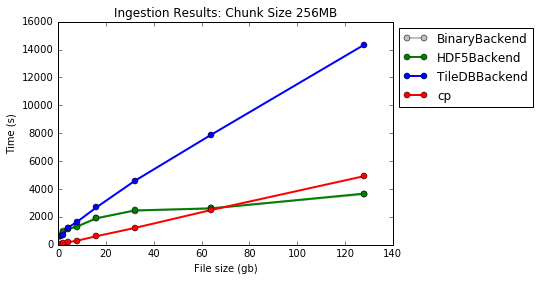
\includegraphics[scale=.75]{./img/ingestion-exp.png}
\caption{Total runtime for different backend implementations in the ingestion
  experiment.}
\label{fig:ingestion-exp}
\end{center}
\end{figure}

As Figure~\ref{fig:ingestion-exp} shows, the \c{HDF5Backend} and
\c{BinaryBackend} scale much more efficiently than the \c{TileDBBackend}. Since
the ingestion experiment is a write heavy workload, the figure shows both the
overall performance as file size increases and speed of writes in the system.
Since the \c{TileDBBackend} scales linearly with the file size, we assume that writes
in this system are much more expensive than the others. \\

When writing the \c{TileDBBackend}, we optimized writes by writing the data in
sorted order. If the data is unsorted, TileDB will internally sort the dataset,
thus we want to avoid incurring this overhead during writes. The only other
clues for the large performance gap would be that the data ingested is dense
and not sparse data, which TileDB is optimized for.

\subsection{Precompute Experiment}\label{storage-ch:precompute-exp}

The precomputation experiment calculates the spectrogram for a given \c{mrn} We
use the same file sizes as in the ingestion experiment, using the ingested data
for this calculation of the spectrogram. Similarly to the ingestion experiment,
we vary the chunk sizes for writing the spectrogram back to the
\c{StorageBackend}. In the evaluation, we use the same chunk size as the
ingestion experiment, 256MB. \\

For this experiment, we evaluate the read time, write time, and total time
across the different \c{StorageBackend} implementations. The read time is
calculated as the sum of all reads across regions when producing the
spectrogram. Similarly, the write time is compute as the total time to write
the calculated spectrogram values across all regions. The total time accounts
for the read and write times in addition to the FFT calculation for computing
the spectrogram.

\subsubsection{Read Time}

\begin{figure}[h]
\begin{center}
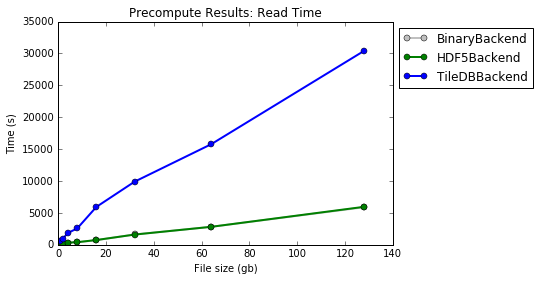
\includegraphics[scale=0.75]{./img/precompute-exp-read-time.png}
\caption{Total read time for different backend implementations in the
  precompute experiment.}
\label{fig:precompute-exp-read-time}
\end{center}
\end{figure}

As Figure~\ref{fig:precompute-exp-read-time} shows, both the \c{BinaryBackend}
and \c{HDF5Backend} have similar read times, with a near constant value
across file sizes. The \c{TileDBBackend} on the otherhand has a growing read
time between processing 32GB and 128GB files. The runtime for the
\c{TileDBackend} is also an order of magnitude greater than the other systems. \\

One possibility for the large performance gap here could be the way TileDB
internally reads data from the disk. The \c{BinaryBackend} takes the entire
memory chunk it reads and interprets it as an array of \c{float} values. Given
the performance similarity to the \c{HDF5Backend}, we can assume a similar
computation is done when extracting data from HDF5. TileDB on the otherhand
reads each cell from memory and converts it to a floating point value. This
pass over the memory manually converting each time could be one reason for the
poor read performance.

\subsubsection{Write Time}

\begin{figure}[h]
\begin{center}
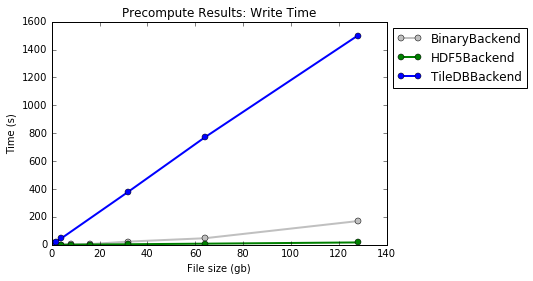
\includegraphics[scale=0.75]{./img/precompute-exp-write-time.png}
\caption{Total write time for different backend implementations in the
  precompute experiment.}
\label{fig:precompute-exp-write-time}
\end{center}
\end{figure}

Similar to Figure~\ref{fig:ingestion-exp},
Figure~\ref{fig:precompute-exp-write-time} shows that the \c{TileDBBackend}
scales linearly with the filesize while the HDF5 and Binary implementations can
write in almost constant time. Since TileDB writes each cell individually, it's
possible, as with reading, this factor causes high write times. \\

The \c{HDF5Backend} outperforms the \c{BinaryBackend} slightly for large
inputs, it's possible this difference is caused by HDF5 buffering writes as
the \c{BinaryBackend} does not.

\subsubsection{Total Time}

\begin{figure}[h]
\begin{center}
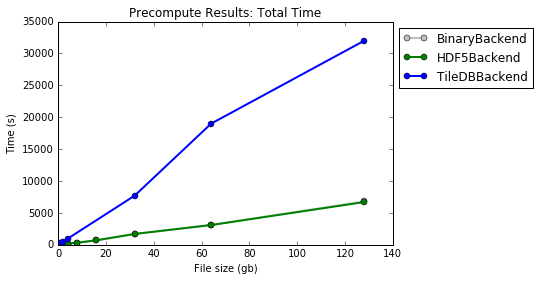
\includegraphics[scale=0.75]{./img/precompute-exp-total-time.png}
\caption{Total runtime for different backend implementations in the precompute
  experiment.}
\label{fig:precompute-exp-total-time}
\end{center}
\end{figure}

We show the total runtime of the precompute program in
Figure~\ref{fig:precompute-exp-total-time}. We can see that the total time is
dominated by reading the data, with a small amount of time for processing the
FFT across the data windows.

\subsection{Storage Overhead}

In this section we discuss the storage overhead for using each
\c{StorageBackend} type. We define this overhead as any additional disk space
required aside from the desired size of the file. As
Table~\ref{table:storage-overhead} shows, TileDB incurs a large overhead. This
overhead is primarily because of the storing the coordinate values (the $(i,j)$
coordinates within the matrix). TileDB does have some bookkeeping structures,
however these are of constant size for a given array. We allow TileDB to GZIP
the coordinate values to reduce the overhead, but there is currently no
mechanism to remove them entirely. \\

The \c{BinaryBackend} has a $0\%$ overhead because each file only has an additional
80 bytes to store the header information. Similarly, HDF5 has a small overhead,
for internal data structures describing the array.

\begin{table}[h!]
\centering
 \begin{tabular}{|c |c |c |c|}
  \hline
  \c{StorageBackend} & Max. Overhead ($\%$) & Avg. Overhead ($\%$) \\
  \hline
  \c{BinaryBackend} & $0$ & $0$ \\
  \hline
  \c{HDF5Backend} & $2.4$ & $1.5$ \\
  \hline
  \c{TileDBBackend} & $38$ & $38$ \\
  \hline
\end{tabular}
\caption{Storage overhead costs for each \c{StorageBackend} type.}
\label{table:storage-overhead}
\end{table}

